\documentclass[12pt,twoside,openright]{report}
\usepackage{minted}
\usepackage{xcolor}
\definecolor{light-gray}{rgb}{0.9,0.9,0.9}
\usepackage{emptypage}
\usepackage[T1]{fontenc}
\usepackage{textcomp}
\usepackage[utf8]{inputenc}
\usepackage[italian]{babel}
\usepackage{graphicx}
\graphicspath{ {immagini/} }
\usepackage{caption}
\usepackage{subcaption}
\usepackage[a4paper,width=150mm,top=30mm,bottom=30mm,left=30mm,right=30mm,bindingoffset=6mm]{geometry}
\usepackage{fancyhdr}
\pagestyle{fancy}
\setlength{\headheight}{15pt}% 
\fancyhead{}
\fancyhead[RE, LO]{\leftmark}
\fancyfoot{}
\fancyfoot[LE,RO]{\thepage}
\renewcommand{\headrulewidth}{0.4pt}
\renewcommand{\footrulewidth}{0.4pt}
\linespread{1.5}\selectfont

\begin{document}

  \shipout\null  

  \thispagestyle{plain}
\chapter*{Abstract}

Il continuo sviluppo delle tecnologie di apprendimento automatico ha reso più semplice ed efficace il monitoraggio dei dati relativi alla salute dell’uomo. L’obiettivo di questa tesi è quello di estrarre ed elaborare informazioni a partire da immagini dell’iride al fine di poterle utilizzare come strumento diagnostico. Il software è composto da due parti, la prima legata all’elaborazione dell’immagine, in particolare applicazione di filtri adeguati e metodi di riconoscimento, segmentazione e scaling dell’iride. La seconda parte rielabora i dati ricavati precedentemente al fine di poterli utilizzare in opportuni algoritmi di machine learning. L'implementazione proposta utilizza come strumento di apprendimento automatico una Convolutional Neural Network (CNN) per studiare la veridicità dell’iridologia, una tecnica alternativa di diagnosi che si basa sull’analisi di sezioni dell’iride.

  
  \tableofcontents
  
  \chapter{Introduzione}
  Negli ultimi anni l’analisi dell’occhio si è rivelata particolarmente interessante in diversi ambiti, quali sicurezza, scanner biometrici, identificazione di persone, medicina, etc. In particolar modo l’iride è la porzione dell’occhio che contiene la maggior parte delle informazioni utili a fini scientifici. 

In questo progetto di tesi si esplorano le diverse tecniche di elaborazione di immagini dell’occhio al fine di individuare ed estrapolare regioni di interesse dell’iride (settori di iride chiamati ROI). Lo scopo finale è quello di utilizzare queste regioni come dato fondamentale per effettuare analisi di vario tipo con un approccio alternativo; tuttavia di per sé le zone d’interesse trovate non risultano sufficienti a tale scopo, è necessario dunque inserire un ulteriore metodo che analizzi queste regioni in modo tale da produrre una valutazione il più possibile accurata. Come metodo di valutazione si è pensato di cercare uno strumento che fosse in grado di riconoscere i pattern comuni all’interno dei segmenti precedentemente individuati. La scelta è immediatamente ricaduta su una branca dell’intelligenza artificiale in rapido sviluppo, il machine learning. Esistono infatti opportuni modelli particolarmente adatti a questo problema. Tali modelli saranno approfonditi in seguito in questa trattazione, illustrandone le potenzialità e il funzionamento. L’impiego combinato di tecnologie di apprendimento automatico e di analisi/elaborazione delle immagini risulta quindi efficace per la creazione di modelli che producano, partendo da semplici immagini dell’occhio, una analisi accurata in modo automatico. 

Il caso d’uso preso in considerazione per lo studio e l’applicazione dei metodi di elaborazione di immagini e degli algoritmi di machine learning è quello dell’iridologia, una teoria medica non ancora validata. L’obiettivo finale vuole essere quello di confrontare i risultati ottenuti da un modello adeguatamente accurato, creato sulla base delle immagini dell’iride, con quelli sostenuti dell'iridologia al fine di confermare la veridicità o meno della suddetta teoria. 

 

  
  \chapter{Iridologia}
  L’iridologia è una pratica pseudoscientifica di diagnosi basata sull’osservazione dell’iride.  È considerata una medicina alternativa in quanto non esiste alcun riscontro medico/scientifico che convalidi le sue teorie.  Secondo l’iridologia, l’iride è divisa in specifiche sezioni che corrispondono a specifiche parti del corpo. Le immagini seguenti rappresentano la mappa delle zone d’interesse creata dal Dr. Bernard Jensen, uno dei pionieri della teoria.

\begin{figure}[h]
  \centering
  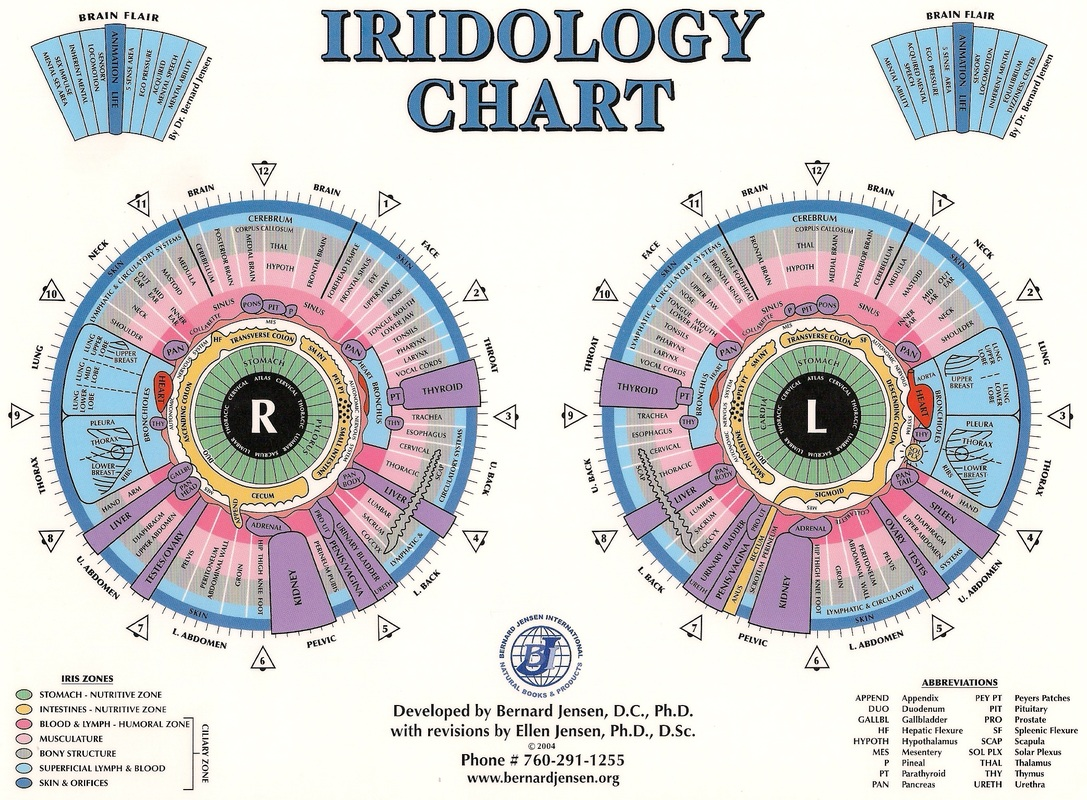
\includegraphics[scale=0.7]{iridology_chart}
  \caption{Mappa dell'iride del Dr. Bernard Jensen}
\end{figure}

Nella mappa sono state individuate 166 aree di cui 80 nell’iride destra e 86 in quella sinistra. Gli iridologi sostengono che guardando una particolare sezione dell’iride, in accordo alla mappa sopracitata, si può determinare, anche in assenza di sintomi, l’esistenza o meno di un problema nella regione del corpo relativa al segmento in esame; tuttavia la teoria non definisce quale sia la presunta malattia. Nella pratica gli iridologi generalmente usano strumenti come microscopi o lenti di ingrandimento per verificare cambiamenti nell’iride, in particolare si cercano specifici pattern di colori o irregolarità nel tessuto dell’occhio. I risultati sono poi comparati con la mappa per correlare le zone affette ai relativi organi. Quindi tutto ciò significa che un’eventuale malattia si dovrebbe riflettere in un evidente cambiamento in qualche sezione dell’iride. Molti studi tuttavia hanno dimostrato che non c’è diretta correlazione tra malattia e iride ed è per questo che la maggior parte dei dottori rigetta questa teoria. 

  
  \chapter{Machine Learning applicato all'iridologia}
  Nel seguente progetto si è cercato di utilizzare un approccio alternativo alle classiche ricerche mediche per dare un parere relativo alla veridicità o meno dell’iridologia. Si è pensato di utilizzare il Machine Learning: esso è lo studio scientifico di algoritmi che creano modelli matematico-statistici, basati sull’inferenza e la ricerca di pattern nei dati, affinché una macchina possa effettuare previsioni senza che venga esplicitamente programmata per farlo. L’accuratezza di tali previsioni è legata al processo di ricerca dei pattern sopracitato, detto anche processo di training: il modello apprenderà le variazioni tra questi dati di training e le utilizzerà per capire quale previsione dare in output a fronte di un nuovo dato. La precisione di queste previsioni sarà quindi strettamente legata ai dati su cui si fa training del modello in riferimento alla quantità e qualità di essi. L’approccio alternativo si basa sull’utilizzo di un modello, opportunamente accurato, che sia in grado, partendo da un segmento di iride legato ad una parte del corpo secondo la mappa dell’iridologia, di produrre in output una predizione riguardo la presenza o meno di un problema relativo alla parte del corpo associata al suddetto segmento. In questo modo si può confrontare il risultato prodotto dal modello con il parere di un iridologo; se nella maggior parte dei casi i pareri risultano discordanti significa che, con buona probabilità, non c’è una correlazione diretta tra iride e patologia. 

Tuttavia è doveroso fare alcune premesse: il modello utilizzato, al fine di produrre previsioni il più possibile corrette, deve avere una buona accuratezza; inoltre, per garantire la validità delle previsioni, è necessario fare training su immagini che abbiano una vera validità medica. Ad esempio: se si vuole cercare il riscontro di un problema al cuore sull’iride, bisogna fare training con segmenti relativi alla sezione dell’iride dedicata al cuore sia di persone di cui si conosce per certo l’esistenza di un problema al cuore sia di persone che non hanno nessun problema all’organo. In questo modo il modello imparerà a capire se vi è una relazione tra porzione di iride e problema al cuore. Una predizione prodotta dal modello ed una valutazione fatta da un iridologo possono poi essere confrontata con il parere di un medico professionista per avere un riscontro oggettivo. Per poter ottenere questo obiettivo si è ricercato un modello che fosse in grado di analizzare immagini al fine di capirne i pattern. Il modello più idoneo per questo tipo di problema è quello delle Convolutional Neural Network (CNN), una sottoclasse di modelli di machine learning dette Artificial Neural Network. Una descrizione più dettagliata delle CNN verrà trattata nel capitolo 6.2.


  
  \chapter{Struttra del progetto}
  \section{Tecnologie}
  Per la realizzazione dell’intero progetto si è utilizzato come linguaggio di programmazione Python 3. Si è scelto questo linguaggio per diversi motivi, il primo in assoluto è relativo al fatto che python rappresenta il linguaggio maggiormente utilizzato nello sviluppo di applicazioni legate al mondo del Machine Learning, difatti i più moderni framework per l’apprendimento automatico, come Tensorflow ad esempio, sono sviluppati in python. Tuttavia, questo non è l’unico motivo, anzi, ci sono altre ragioni che hanno portato alla scelta di questo linguaggio, ad esempio altri punti di forza di python sono la semplicità, la flessibilità e la versatilità, è infatti disponibile sulle principali piattaforme in circolazione (Windows, Linux e Mac OS). Altre caratteristiche sono il supporto di più paradigmi, tra cui: object oriented, strutturale e funzionale e la grande disponibilità di moduli pronti all’uso che permettono di arricchire il set di funzioni base del linguaggio. 
Tra i diversi moduli utilizzati nell’applicativo i principali sono:
\begin{itemize}
  \item \textbf{Python - OpenCV (cv2)}:  OpenCV sta per Open Source Computer Vision Library; Python - OpenCV è la versione python della popolare libreria utilizzata per la visione artificiale. Nel progetto viene utilizzata per le varie funzioni di elaborazione delle immagini
  \item \textbf{Numpy}: questa libreria aggiunge al linguaggio il supporto di array multidimensionali e matrici anche di grandi dimensioni; inoltre aggiunge anche molte funzioni matematiche di altro livello utili per operare con questo tipo di dati
  \item \textbf{Tensorflow}: framework sviluppato per l’apprendimento automatico. Contiene una vasta gamma di funzionalità legate al mondo del Machine Learning, fornisce moduli ottimizzati per la realizzazione di algoritmi o modelli di ML. Nell’ applicativo viene utilizzato soprattutto per la creazione della rete neurale
  \item \textbf{ConfigParser}: libreria che implementa un file parser per gestire file di configurazione strutturati
  \item \textbf{os}: modulo nativo di python che permette di utilizzare funzioni del sistema operativo. Ad esempio nel progetto viene spesso utilizzato per fare controlli su file, creare/eliminare cartelle e gestire path
\end{itemize}


  \section{Struttura del codice}
  Il progetto è composto da una serie di script python; la maggior parte è organizzata in moduli, ovvero collezioni di script che contengono solo funzioni o costanti, oltre a questi file sono anche presenti tre script direttamente eseguibili che richiamano le funzioni offerte da tali moduli.

I due moduli creati sono:
\begin{itemize}
  \item \textbf{Preprocessing}: contiene gli script necessari alla fase preparazione dei dati per il training della rete neurale. In particolare contiene tutte le funzioni per l’elaborazione delle immagini, come filtri, metodi di riconoscimento dell’iride, etc...
  \item \textbf{ML\_CNN}:  contiene gli script che permettono di creare, fare training e deploy del modello di rete neurale  
\end{itemize}

Gli script principali, ovvero quelli che poi verranno effettivamente mandati in esecuzione,  sono tre: \texttt{preprocess.py}, \texttt{train.py} e \texttt{predict.py}. \texttt{Preprocess.py} richiama le funzioni offerte dal modulo Preprocessing per elaborare le immagini in input al fine di  creare in output le immagini del segmento di iride selezionato. Lo script \texttt{train.py} utilizza le funzioni offerte dal modulo ML\_CNN per creare il dataset di training partendo dai segmenti precedentemente generati; successivamente, richiama i metodi per la generazione e il training del modello, producendo infine in output un file con estensione \texttt{.model} che rappresenta il modello appena creato. Infine lo script \texttt{predict.py} riutilizza il modulo Preprocessing per elaborare le nuove immagini su cui si vuole fare una previsione, così da produrre a sua volta i segmenti di iride. Si usa infine il modello scelto dall’utente e si producono in output le previsioni  generate dalla rete neurale.

  \section{File di configurazione}
  Dato che le diverse funzioni nel codice contengono svariati parametri di configurazione si è pensato di creare un apposito file contenente le associazioni parametro-valore, chiamato \texttt{config.ini}. Il file è strutturato in sezioni ed ogni sezione ha associato un insieme di parametri ad essa relativi; questi rappresentano i parametri fondamentali di tutte le principali funzioni presenti nel programma. Lo scopo di questo file è creare un metodo più rapido e semplice per la modifica dei valori dei parametri, in questo modo un utente che vuole effettuare test diversi, non necessariamente riguardanti l’iridologia, può semplicemente andare a modificare i valori dei parametri di interesse senza dover modificarli direttamente nelle chiamate alle funzioni nel codice.

  
  \chapter{Premesse}
  E’ necessario fare una serie di premesse riguardo la scelta delle immagini da utilizzare nel programma, la quale risulta fondamentale per il corretto funzionamento dello stesso. Le immagini che verranno processate e successivamente utilizzate nel modello di training devono avere la stessa dimensione (non troppo piccola), in quanto dimensioni differenti porterebbero ad avere errori nel riconoscimento dell’iride e della pupilla. Le foto dell’occhio devono essere scattate frontalmente, poiché il programma non è sempre in grado di riconoscere l’iride se l’occhio è trasversale. E’ inoltre molto importante che l’occhio sia ben aperto, limitando il più possibile la presenza delle palpebre, in quanto risulterebbe falsata l’analisi di un segmento che le contiene anche solo parzialmente. 

\begin{figure}
  \centering
  \begin{subfigure}[b]{0.4\textwidth}
    \centering
    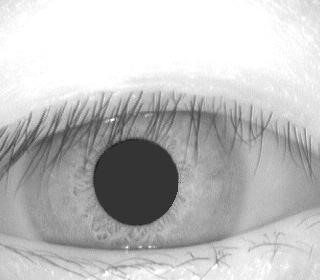
\includegraphics[width=\textwidth]{premesse_1}
    \caption{Immagine non ottimale}    
  \end{subfigure}
  \hfill
  \begin{subfigure}[b]{0.4\textwidth}
    \centering
    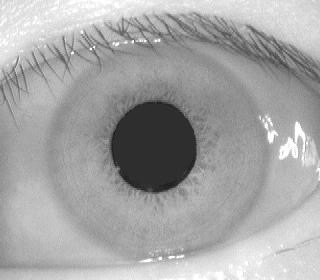
\includegraphics[width=\textwidth]{premesse_2}
    \caption{Immagine ottimale}       
  \end{subfigure}
  \caption{Esempi di immagini presenti nel dataset CASIA}
\end{figure}

Inoltre affinché un modello di machine learning produca risultati attendibili nel caso d’uso trattato, si dovrebbe utilizzare idealmente un elevato numero di immagini, equamente distribuite nelle classi di training. Un’ultima, importante premessa, va fatta riguardo il file di configurazione. In esso i parametri  sono settati appositamente per l’implementazione proposta. L’utilizzo di immagini differenti, in particolar modo di dimensioni diverse da quelle del dataset utilizzato in questo lavoro, comporta una dovuta modifica di alcuni di questi parametri, a carico dell’utente. Se non vengono modificati correttamente, i risultati dell’elaborazione potrebbero portare allo scarto di numerose immagini in seguito, ad esempio,  alla non corretta identificazione dei segmenti. 

  
  \chapter{Panoramica del processo di funzionamento}
  Di seguito verrà fatta una descrizione generalizzata del processo di funzionamento del software, mentre nei capitoli successivi si andranno a descrivere più nel dettaglio le singole parti del codice che portano all’obiettivo finale. Il codice è suddiviso in tre macro-sezioni: la sezione di elaborazione delle immagini, la sezione dedicata al machine learning e infine la sezione che si occupa di effettuare le previsioni. Come prima cosa, l’utente inserisce le immagini su cui fare training nella cartella \texttt{DATA\_IMAGES}, in particolare suddivide le immagini in due subset: il set di immagini associate ad un problema andranno inserite nella sottocartella \texttt{DB\_PROBS} mentre il set di immagini che si possono definire senza problematiche va inserito nella sottocartella \texttt{DB\_NORMAL}. Una volta inseriti i dati si può procedere all’esecuzione dello script \texttt{preprocess.py}: tale script, come già anticipato, carica le immagini collocate nella cartella \texttt{DATA\_IMAGES} e successivamente richiama diverse funzioni di elaborazione delle immagini. Le immagini processate vengono poi inviate alle funzioni di riconoscimento di iride e pupilla, quelle con un riscontro positivo passano poi alla funzione di segmentazione e crop, infine si procede al resize dei segmenti ad una dimensione fissa e al salvataggio. Alla fine di questo sottoprocesso lo script crea nella cartella root del progetto una sottocartella chiamata \texttt{TEMP\_SEG}, contenente a sua volta due sottocartelle chiamate \texttt{DB\_NORMAL\_SEG} e \texttt{DB\_PROBS\_SEG}. All’interno di esse troviamo rispettivamente i segmenti di iride elaborati relativi  alle immagini in \texttt{DB\_NORMAL} e in \texttt{DB\_PROBS}. E’ importante notare che nel caso di errori durante la fase di “filtraggio” delle immagini oppure nel caso di errori dovuti alla mancata rilevazione o rilevazione errata dell’iride/pupilla (intesa come rilevazione di più di un’iride/pupilla)  il programma provvede a scartare l’immagine; quindi il numero segmenti in output potrebbe risultare inferiore di quello delle immagini in input. Una volta generati i segmenti si procede con il training della rete neurale. Per far ciò si manda in esecuzione lo script \texttt{train.py}, che carica le immagini dei segmenti e li organizza in una struttura dati che può essere analizzata dalla rete. Una volta ottenuta tale struttura si può passare alla creazione del modello e al training vero e proprio, al termine di tale processo lo script produce in output il file \texttt{.model} che contiene tutte le informazioni relative al modello appena generato. Il modello può essere poi utilizzato nella fase finale, ovvero nella fase di prediction, per fare previsioni. L’utente andrà ad inserire nella cartella \texttt{DATA\_TO\_PREDICT}, sottocartella di \texttt{PREDICTION}, le immagini di cui vuole una previsione, poi inserisce nella cartella \texttt{PREDICTION} il file \texttt{.model} relativo al modello di rete neurale che si vuole utilizzare per fare la previsione. Fatta questa preparazione si esegue lo script \texttt{predict.py} che fa passare le immagini presenti nella cartella \texttt{DATA\_TO\_PREDICT} attraverso le fasi di preprocessing in modo da produrre dei segmenti utilizzabili dal modello preso in esame (in sostanza produce dei segmenti della stessa dimensione dei segmenti usati per fare il training del modello). Infine lo script carica in memoria il modello e chiede alla rete di fare previsioni sui segmenti precedentemente creati, in output l’utente si ritroverà la label (problema o normale) che la rete ha ritenuto opportuno associare a quel segmento. La descrizione appena fatta rappresenta un utilizzo tipico del programma, tuttavia è importante menzionare il fatto che non è obbligatorio fare un’esecuzione sequenziale delle tre macro-sezioni; infatti è possibile per esempio eseguire \texttt{predict.py} su modelli diversi e non necessariamente sull’ultimo modello creato. Di seguito si andrà a fare un descrizione dettagliata delle diverse fasi del processo, relative allo specifico caso d’uso dell’iridologia,  che partendo dalle immagini di input portano alle predizioni finali. E’ doveroso far notare che per poter procedere nella realizzazione dell’elaborato, non avendo a disposizione immagini strettamente legate all’iridologia, si è scelto di utilizzare il dataset CASIA v.4.0, il quale è composto quasi interamente da immagini che soddisfano tutte le premesse fatte in precedenza ma che tuttavia contiene solo immagini di occhi normali (a cui non è associato nessun problema) e quindi non rappresenta un valido dataset per verificare la validità dell’iridologia. Di conseguenza i risultati di training non saranno accurati, ma per l’elaborazione delle immagini ed estrazione dei segmenti il dataset scelto si è rivelato ottimale. Per questo motivo è doveroso dire che il programma non è stato pensato e scritto solo per il caso d’uso dell’iridologia, ma è potenzialmente utilizzabile per ulteriori progetti relativi all’analisi dell’occhio, infatti si presuppone che con le adeguate immagini, categorizzate in modo opportuno, si riescano ad ottenere dei buoni risultati. Detto ciò, le immagini presenti in questo dataset (in seguito alla cancellazione di alcune immagini non soddisfacenti le premesse) sono 488. Si farà spesso riferimento a parametri scelti appositamente per questo caso d’uso, tarati in base alle immagini a disposizione.

  
  \chapter{Elbaorazione delle immagini}
  All’avvio dello script \texttt{preprocess.py} viene inocata la funzione \texttt{create\_data} che si occupa di estrarre i segmenti dalle immagini in input, tale risultato è ottenuto invocando una serie di altre funzioni in sequenza che verranno descritte di seguito.

  \section{Caricamento delle immagini}
  La prima funzione è \texttt{load\_image}, si occupa di caricare le immagini presenti nel path passato come parametro e le restituisce come un array di immagini (matrici di pixel). Il path è preimpostato e punta alla cartella \texttt{DATA\_IMAGES} che , come già accennato in precedenza, contiene il dataset di immagini CASIA divise per tipologia. Il caricamento viene reso possibile dalla funzione \texttt{cv2.imread} della libreria OpenCV che carica le immagini come matrici di pixel codificate nel formato BGR (Blue Green Red). Qualora fosse necessario è possibile abilitare a \texttt{True} il parametro \texttt{RESIZE} presente nella sezione \texttt{PREPROCESSING} del file di configurazione,in questo modo viene effettuato un resize automatico sulla base della dimensioni specificate dal parametro \texttt{RESIZE\_SHAPE}, nel nostro caso non è stato necessario fare un resize in quanto tutte le immagini erano già della stessa dimensione (320 x  280). La funzione ritorna l’array di matrici a tre livelli contenenti i valori BGR dei pixel delle immagini e l’array contenente i nomi dei file delle immagini.

  \section{Filtri}
  All’avvio dello script \texttt{preprocess.py} viene inocata la funzione \texttt{create\_data} che si occupa di estrarre i segmenti dalle immagini in input, tale risultato è ottenuto invocando una serie di altre funzioni in sequenza che verranno descritte di seguito.

  \subsection{Trasformazioni morfologiche}
  Una trasformazione morfologica è una semplice operazione  basata sulla shape (high x width) dell’immagine.


\begin{minted}
[
  xleftmargin=\parindent,
  framesep=2mm,
  baselinestretch=1.2,  
  fontsize=\footnotesize,
  linenos
]
{python}

kernel = cv2.getStructuringElement(cv2.MORPH_ELLIPSE, (5, 5))
blackhat = cv2.morphologyEx(cimg, cv2.MORPH_BLACKHAT, kernel)
bottom_hat_filtered = cv2.add(blackhat, cimg)    
\end{minted}

Nel codice sopra riportato la funzione che opera le trasformazioni morfologiche è \texttt{cv2.morphologyEx}, la quale utilizza erosione e dilatazione come operazioni di base. L’erosione consiste nell’erodere i bordi di una forma, un pixel nell’immagine originale in bianco e nero (0 o 1) sarà considerato 1 solo se tutti i pixels coperti dal kernel sono 1, altrimenti è eroso (messo a zero). La dilatazione invece effettua il processo inverso dell’erosione. MorphologyEx necessita di due input, il primo è l’immagine originale, il secondo è chiamato structuring element o kernel. Specificando come parametro della funzione \texttt{cv2.getStructuringElement MORPH\_ELLIPSE} si ricava un elemento strutturale a forma di ellisse inscritta in un rettangolo, tale elemento viene poi utilizzato come kernel effettivo per ricavare il blackhat. Questo tipo di operazione mette in risalto regioni scure dell’immagine con uno sfondo luminoso. Il passo finale è l’applicazione del blackhat all’immagine in grayscale, il risultato è chiamato bottom hat.


\begin{figure}[h]
  \centering
  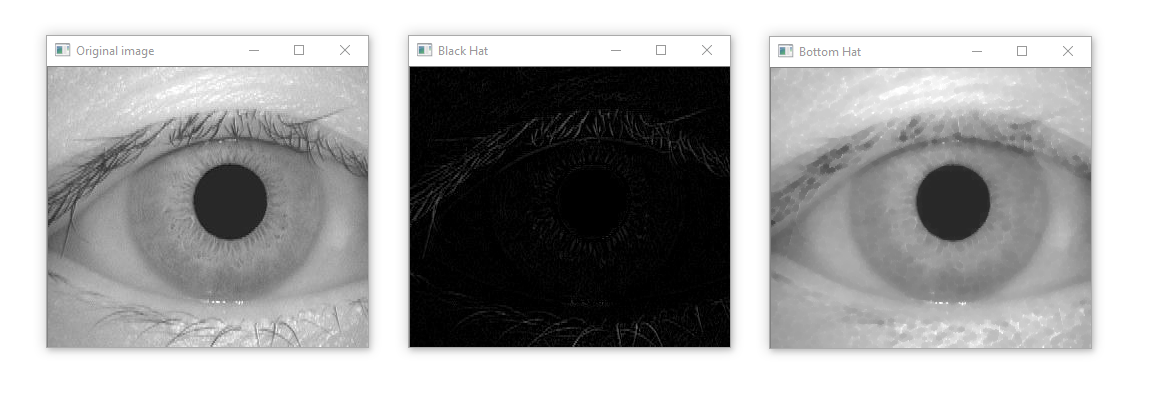
\includegraphics[width=1.0\textwidth]{black_hat}
  \caption{Applicazione della trasformazione black hat all'immagine}
\end{figure}

La scelta di queste trasformazioni morfologiche risiede nel fatto che si adattano molto bene alla successiva applicazione di un blur, in particolar modo del Gaussian Blur.

\end{document}
